% Created by tikzDevice version 0.12.6 on 2026-08-03 03:41:23
% !TEX encoding = UTF-8 Unicode
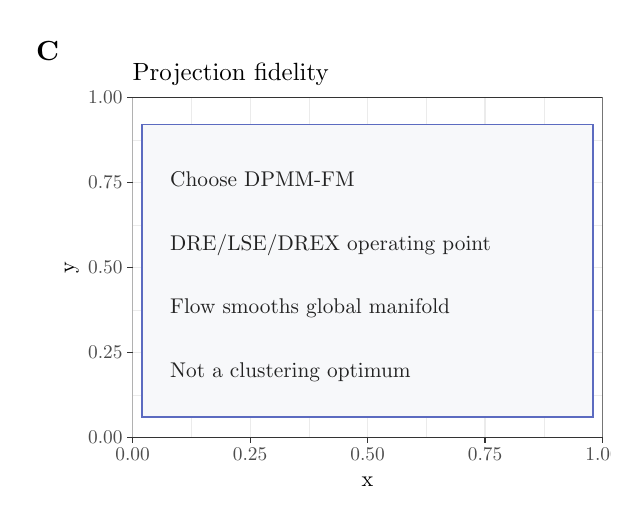
\begin{tikzpicture}[x=1pt,y=1pt]
\definecolor{fillColor}{RGB}{255,255,255}
\path[use as bounding box,fill=fillColor,fill opacity=0.00] (0,0) rectangle (210.78,171.36);
\begin{scope}
\path[clip] (  1.05,  1.87) rectangle (209.73,169.49);
\definecolor{drawColor}{RGB}{255,255,255}
\definecolor{fillColor}{RGB}{255,255,255}

\path[draw=drawColor,line width= 0.4pt,line join=round,line cap=round,fill=fillColor] (  1.05,  1.87) rectangle (209.73,169.49);
\end{scope}
\begin{scope}
\path[clip] ( 37.90, 23.34) rectangle (207.73,146.20);
\definecolor{fillColor}{RGB}{255,255,255}

\path[fill=fillColor] ( 37.90, 23.34) rectangle (207.73,146.20);
\definecolor{drawColor}{gray}{0.92}

\path[draw=drawColor,line width= 0.2pt,line join=round] ( 37.90, 38.69) --
	(207.73, 38.69);

\path[draw=drawColor,line width= 0.2pt,line join=round] ( 37.90, 69.41) --
	(207.73, 69.41);

\path[draw=drawColor,line width= 0.2pt,line join=round] ( 37.90,100.12) --
	(207.73,100.12);

\path[draw=drawColor,line width= 0.2pt,line join=round] ( 37.90,130.84) --
	(207.73,130.84);

\path[draw=drawColor,line width= 0.2pt,line join=round] ( 59.13, 23.34) --
	( 59.13,146.20);

\path[draw=drawColor,line width= 0.2pt,line join=round] (101.59, 23.34) --
	(101.59,146.20);

\path[draw=drawColor,line width= 0.2pt,line join=round] (144.04, 23.34) --
	(144.04,146.20);

\path[draw=drawColor,line width= 0.2pt,line join=round] (186.50, 23.34) --
	(186.50,146.20);

\path[draw=drawColor,line width= 0.4pt,line join=round] ( 37.90, 23.34) --
	(207.73, 23.34);

\path[draw=drawColor,line width= 0.4pt,line join=round] ( 37.90, 54.05) --
	(207.73, 54.05);

\path[draw=drawColor,line width= 0.4pt,line join=round] ( 37.90, 84.77) --
	(207.73, 84.77);

\path[draw=drawColor,line width= 0.4pt,line join=round] ( 37.90,115.48) --
	(207.73,115.48);

\path[draw=drawColor,line width= 0.4pt,line join=round] ( 37.90,146.20) --
	(207.73,146.20);

\path[draw=drawColor,line width= 0.4pt,line join=round] ( 37.90, 23.34) --
	( 37.90,146.20);

\path[draw=drawColor,line width= 0.4pt,line join=round] ( 80.36, 23.34) --
	( 80.36,146.20);

\path[draw=drawColor,line width= 0.4pt,line join=round] (122.82, 23.34) --
	(122.82,146.20);

\path[draw=drawColor,line width= 0.4pt,line join=round] (165.27, 23.34) --
	(165.27,146.20);

\path[draw=drawColor,line width= 0.4pt,line join=round] (207.73, 23.34) --
	(207.73,146.20);
\definecolor{drawColor}{RGB}{92,107,192}
\definecolor{fillColor}{RGB}{247,248,250}

\path[draw=drawColor,line width= 0.5pt,fill=fillColor] ( 41.29, 30.71) rectangle (204.34,136.37);
\definecolor{drawColor}{RGB}{34,34,34}

\node[text=drawColor,anchor=base west,inner sep=0pt, outer sep=0pt, scale=  0.77] at ( 51.48,113.88) {Choose DPMM-FM};

\node[text=drawColor,anchor=base west,inner sep=0pt, outer sep=0pt, scale=  0.77] at ( 51.48, 90.94) {DRE/LSE/DREX operating point};

\node[text=drawColor,anchor=base west,inner sep=0pt, outer sep=0pt, scale=  0.77] at ( 51.48, 68.01) {Flow smooths global manifold};

\node[text=drawColor,anchor=base west,inner sep=0pt, outer sep=0pt, scale=  0.77] at ( 51.48, 45.08) {Not a clustering optimum};
\definecolor{drawColor}{gray}{0.20}

\path[draw=drawColor,line width= 0.4pt,line join=round,line cap=round] ( 37.90, 23.34) rectangle (207.73,146.20);
\end{scope}
\begin{scope}
\path[clip] (  0.00,  0.00) rectangle (210.78,171.36);
\definecolor{drawColor}{gray}{0.30}

\node[text=drawColor,anchor=base east,inner sep=0pt, outer sep=0pt, scale=  0.70] at ( 34.30, 20.93) {0.00};

\node[text=drawColor,anchor=base east,inner sep=0pt, outer sep=0pt, scale=  0.70] at ( 34.30, 51.64) {0.25};

\node[text=drawColor,anchor=base east,inner sep=0pt, outer sep=0pt, scale=  0.70] at ( 34.30, 82.36) {0.50};

\node[text=drawColor,anchor=base east,inner sep=0pt, outer sep=0pt, scale=  0.70] at ( 34.30,113.07) {0.75};

\node[text=drawColor,anchor=base east,inner sep=0pt, outer sep=0pt, scale=  0.70] at ( 34.30,143.79) {1.00};
\end{scope}
\begin{scope}
\path[clip] (  0.00,  0.00) rectangle (210.78,171.36);
\definecolor{drawColor}{gray}{0.20}

\path[draw=drawColor,line width= 0.4pt,line join=round] ( 35.90, 23.34) --
	( 37.90, 23.34);

\path[draw=drawColor,line width= 0.4pt,line join=round] ( 35.90, 54.05) --
	( 37.90, 54.05);

\path[draw=drawColor,line width= 0.4pt,line join=round] ( 35.90, 84.77) --
	( 37.90, 84.77);

\path[draw=drawColor,line width= 0.4pt,line join=round] ( 35.90,115.48) --
	( 37.90,115.48);

\path[draw=drawColor,line width= 0.4pt,line join=round] ( 35.90,146.20) --
	( 37.90,146.20);
\end{scope}
\begin{scope}
\path[clip] (  0.00,  0.00) rectangle (210.78,171.36);
\definecolor{drawColor}{gray}{0.20}

\path[draw=drawColor,line width= 0.4pt,line join=round] ( 37.90, 21.34) --
	( 37.90, 23.34);

\path[draw=drawColor,line width= 0.4pt,line join=round] ( 80.36, 21.34) --
	( 80.36, 23.34);

\path[draw=drawColor,line width= 0.4pt,line join=round] (122.82, 21.34) --
	(122.82, 23.34);

\path[draw=drawColor,line width= 0.4pt,line join=round] (165.27, 21.34) --
	(165.27, 23.34);

\path[draw=drawColor,line width= 0.4pt,line join=round] (207.73, 21.34) --
	(207.73, 23.34);
\end{scope}
\begin{scope}
\path[clip] (  0.00,  0.00) rectangle (210.78,171.36);
\definecolor{drawColor}{gray}{0.30}

\node[text=drawColor,anchor=base,inner sep=0pt, outer sep=0pt, scale=  0.70] at ( 37.90, 14.92) {0.00};

\node[text=drawColor,anchor=base,inner sep=0pt, outer sep=0pt, scale=  0.70] at ( 80.36, 14.92) {0.25};

\node[text=drawColor,anchor=base,inner sep=0pt, outer sep=0pt, scale=  0.70] at (122.82, 14.92) {0.50};

\node[text=drawColor,anchor=base,inner sep=0pt, outer sep=0pt, scale=  0.70] at (165.27, 14.92) {0.75};

\node[text=drawColor,anchor=base,inner sep=0pt, outer sep=0pt, scale=  0.70] at (207.73, 14.92) {1.00};
\end{scope}
\begin{scope}
\path[clip] (  0.00,  0.00) rectangle (210.78,171.36);
\definecolor{drawColor}{RGB}{0,0,0}

\node[text=drawColor,anchor=base,inner sep=0pt, outer sep=0pt, scale=  0.80] at (122.82,  5.64) {x};
\end{scope}
\begin{scope}
\path[clip] (  0.00,  0.00) rectangle (210.78,171.36);
\definecolor{drawColor}{RGB}{0,0,0}

\node[text=drawColor,rotate= 90.00,anchor=base,inner sep=0pt, outer sep=0pt, scale=  0.80] at ( 16.86, 84.77) {y};
\end{scope}
\begin{scope}
\path[clip] (  0.00,  0.00) rectangle (210.78,171.36);
\definecolor{drawColor}{RGB}{0,0,0}

\node[text=drawColor,anchor=base west,inner sep=0pt, outer sep=0pt, scale=  0.90] at ( 37.90,152.18) {Projection fidelity};
\end{scope}
\begin{scope}
\path[clip] (  0.00,  0.00) rectangle (210.78,171.36);
\definecolor{drawColor}{RGB}{0,0,0}

\node[text=drawColor,anchor=base,inner sep=0pt, outer sep=0pt, scale=  1.00] at (  7.20,159.49) {\bfseries C};
\end{scope}
\end{tikzpicture}
